\section{Findings}
\label{cha:findings}
% Grading Criteria
% - Steps taken to arrive at the presented findings are clear 
%       => Das kann auch aus dem Background kommen, es muss nur klar sein wie die Ergebnisse zustande kommen
% - The research question is addressed
% - present findings
% - graphs and table support the main findings 
% - findings are presented without judgment

%//TODO captions der bilder sollen nicht achsen beschreiben, sondern information first, da kann ruhig auch ein haufen stehen

\section{How does the k-means Algorithm help to understand Electricity Load Patterns?}
\label{sec:findings_understand_electricity_load_patterns}
Conducting the literature review provided two different options for choosing the value of $k$ before executing k-means:
By choosing a fixed value the clustering results apply to criteria chosen in advance.
Liu et al \cite{LIU-BDE} choose a fixed value of $k=3$ since the clustering results are divided into low-, medium-, and high-consumption clusters.
By applying k-means with a variable value of $k$ the clustering results adapt to the data and therefore deliver problem-specific results.
This enables Jessen et al. \cite{JES-IND} to spot trends in the data without knowing about certain characteristics in advance.
The clustering results of the whole energy-load profile dataset of Lombok, Indonesia, are shown in \ref{fig:whole_data_clustering_results}.
Each cluster holds approximately the data of a single year, for example, the black cluster contains data from 2015 and the red cluster contains mostly data from 2021.
This shows an overall increase in power consumption over the years.
The algorithm also managed to spot different consumption patterns in the data, with the lime cluster containing mostly the Ramadhan periods from 2018 to 2021.

To further improve the overall understanding of the data, further theories and classifications can be applied after executing k-means.
This classification can take place by taking further datasets into account that underline the found characteristics and patterns.
Jessen et al. \cite{JES-IND} algorithmically label the clustering results into "normal" and "abnormal" clusters, with the abnormal clusters being natural disasters or electrical fault impacted.
This is done by comparing the clustering results with the occurrence time and epicenter of natural disasters and electrical faults.
By reapplying the clustering algorithm to the distinct clusters, the labeling process can be proven.
The clustering results for the earthquake-impacted year 2018 are shown in \ref{fig:clustering_results_2018}.
Again, the algorithm divided the data into distinct clusters, with each cluster representing different consumption patterns.
The red cluster contains post-natural disaster data, which is analyzed in greater detail in \ref{fig:clustering_results_2018_cluster_two}.

These findings show, that k-means proves useful in understanding electricity load pattern datasets without prior knowledge.
By applying k-means, characteristics, patterns, and tendencies are spotted within the data.
The clustering results can be adjusted by choosing different values for $k$.
If a certain theory or defined categories want to be proven a fixed value is useful, to generate hidden knowledge out of large datasets a variable value is more useful.
This lays the groundwork for revealing hidden knowledge in the data, enabling more advanced methods to fully grasp the data's meaning.

\begin{figure}
    \centering
    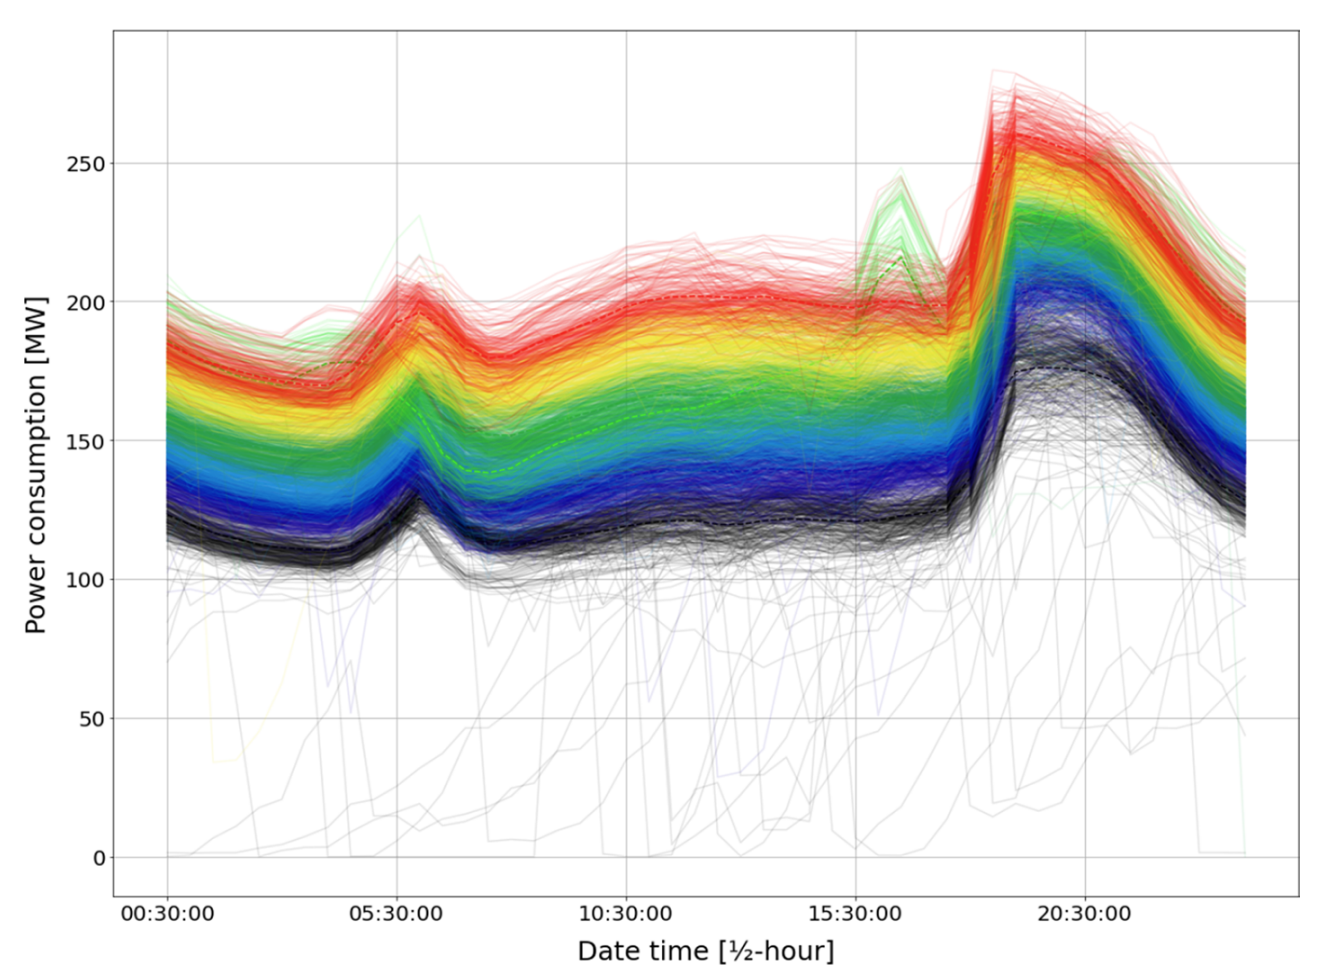
\includegraphics[width=0.8\textwidth]{figures/jessen_ndImpactedClusters/jessen_wholeDataClustering.png}
    \caption{Whole Data Clustering Results \cite{JES-IND};
    Y-Axis: Power Consumption in MW, X-Axis: Time in 30 Minute Intervals;
    Each Cluster is represented by a different color}
    \label{fig:whole_data_clustering_results}
\end{figure}

\begin{figure}
    \centering
    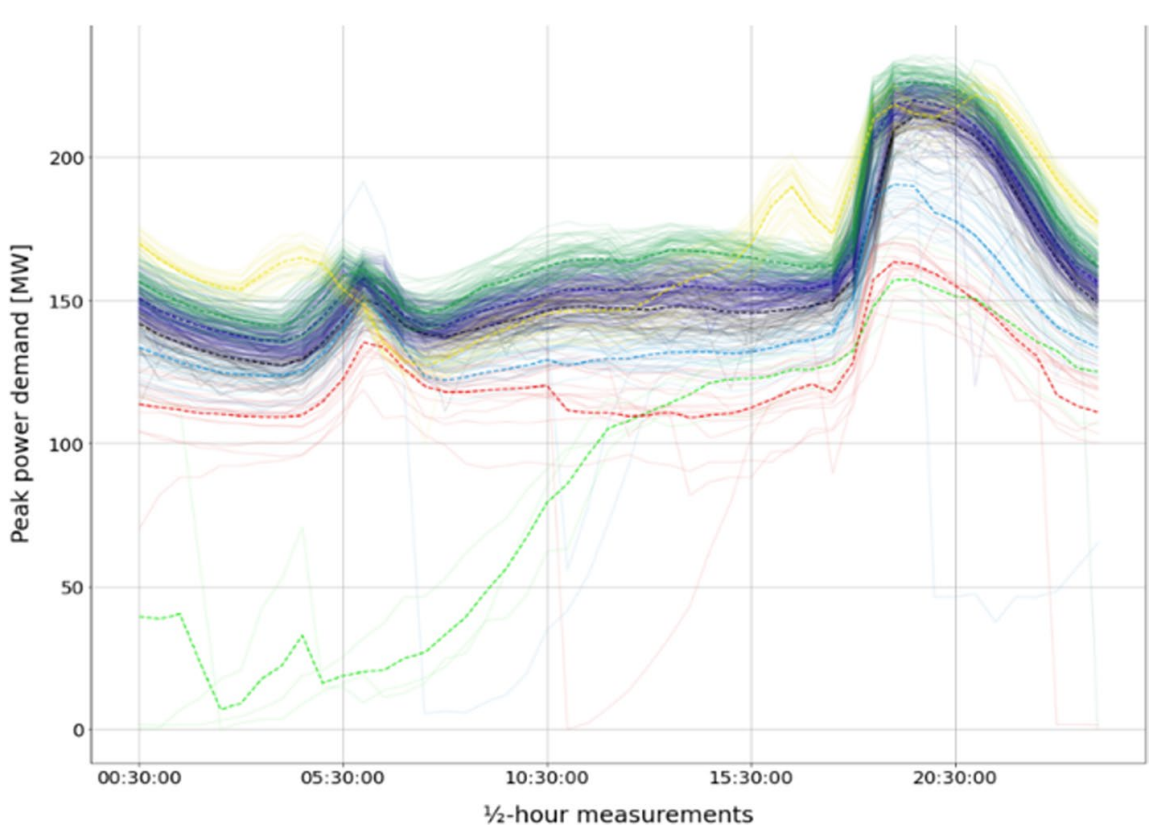
\includegraphics[width=0.8\textwidth]{figures/jessen_ndImpactedClusters/jessen_Clustering2018.png}
    \caption{Clustering Results for the Earthquake-Impacted Year of 2018 \cite{JES-IND};
    Y-Axis: Power Consumption in MW, X-Axis: Time in 30 Minute Intervals;
    Each Cluster is represented by a different color}
    \label{fig:clustering_results_2018}
\end{figure}

\begin{figure}
    \centering
    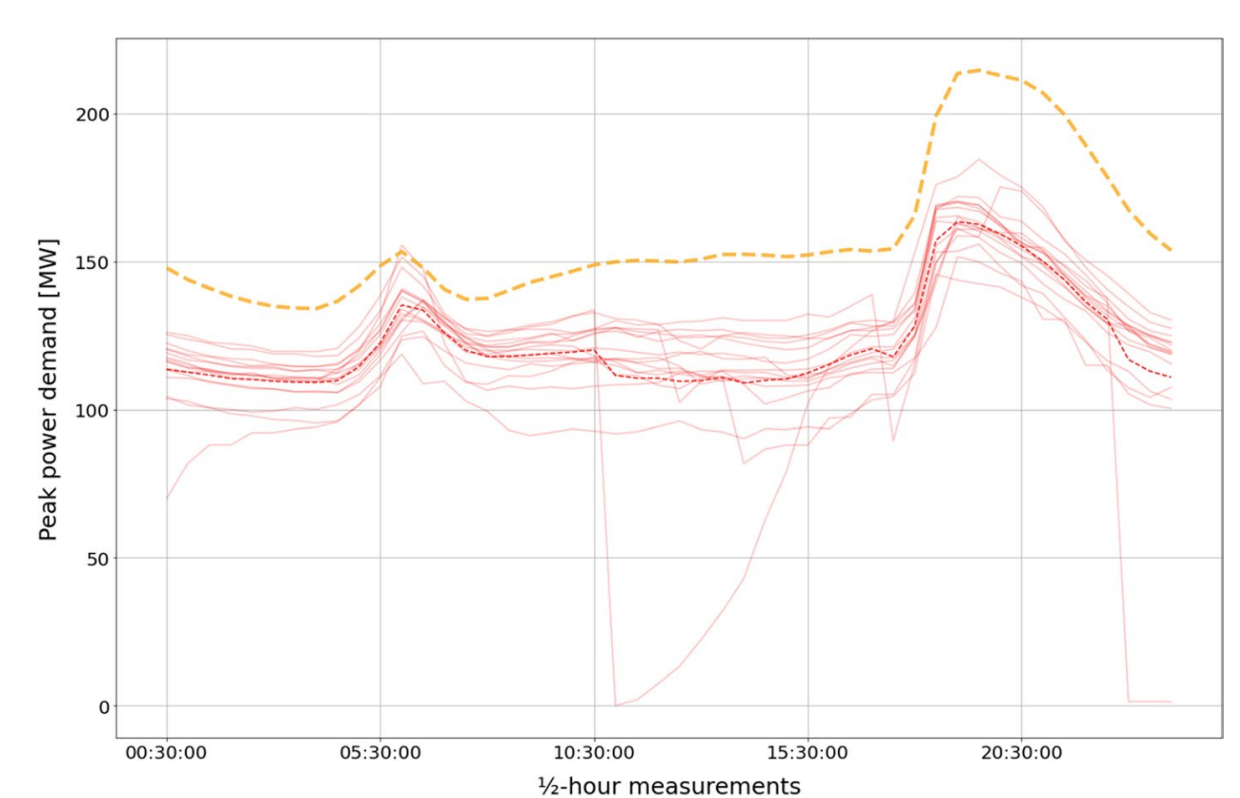
\includegraphics[width=0.8\textwidth]{figures/jessen_ndImpactedClusters/jessen_ClusterTwo2018.png}
    \caption{The Load Profiles in Cluster 2 (16 Samples in total) for Lombok in 2018 \cite{JES-IND};
    The Red Solid Lines represent the Clusters' Daily Profiles, the Red dashed Line is the Average for the Red Cluster, and the thick Orange dashed Line is the daily Average for the whole 2018}
    \label{fig:clustering_results_2018_cluster_two}
\end{figure}

\section{Improving the Design of Energy-Saving Incentives}
\label{sec:improving_the_design_of_energy_saving_incentives}

% Idee So ausführen, dass diese RQ auf der ersten aufbaut => es muss nicht viel neues erklärt werden

% % 1. Allgemeine Ergebnisse ansprechen
% % 2. Auf ein Beispiel eingehen (in diesem Fall das Clustering und die Tabelle)
% The results are separated into four parts: Clustering for freshwater consumption, the environmental performance measured on the sulfur dioxide emissions, and the energy efficiency performance measured on the coal consumption.
% The k-means algorithm is applied multiple times for each part: once for the whole dataset containing all industry sectors and for each industry sector separately.
% Therefore, distinct companies can be assigned to a cluster and be compared with other companies from the same or different industry sectors.
% One of the clustering algorithm's results is shown in \ref{fig:multi_industries_clustering_result_environemental_performance}.
% A certain threshold most companies remain below can be determined.
% Furthermore, the number of companies in each cluster can be counted and compared.
% The results of the assignments for each industry sector according to the environmental performance are shown in \ref{tab:multi_industries_clustering_results_based_on_the_so2_emission}.
% Some industry sectors show a clear tendency towards a specific cluster, while others are less evenly distributed.
% Therefore, general cluster structures can be identified with industry sectors being ranked by the chosen metric.
% Also, companies within industry sectors can be compared, which helps detect outliers and best practices.

\begin{table}[h]
    \centering
    \begin{tabular}{c|c|c|c|c}
        \textbf{Fields} & \textbf{Sum} & \textbf{Cluster 0} & \textbf{Cluster 1} & \textbf{Cluster 2} \\
        \hline
        Chemical Industry & 144 & 138 & 0 & 6 \\
        Coal Mining and Washing Industry & 60 & 54 & 4 & 2 \\
        Black Metal Smelting & 75 & 53 & 6 & 16 \\
        Textile Industry & 49 & 49 & 0 & 0 \\
        Paper Products Industry & 47 & 42 & 0 & 5 \\
        Electricity, Heat Industry & 384 & 274 & 18 & 92 \\
    \end{tabular}
    \caption{Snippet of the Multi-Industries Clustering Results based on the $SO_2$ Emission \cite{LIU-BDE};
    Each Industry Sector is represented by a Row, the Columns represent the Clusters showing the Number of Companies in each Cluster}
    \label{tab:multi_industries_clustering_results_based_on_the_so2_emission}
\end{table}

\begin{figure}
    \centering
    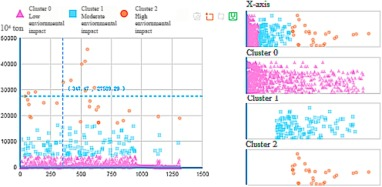
\includegraphics[width=0.8\textwidth]{figures/liu_assessmentOfIndustries/liu_environmentalPerformance.jpg}
    \caption{Multi-Industries Clustering Result based on the $SO_2$ Emission \cite{LIU-BDE};
    Each Point represents a Company its Color represents the Cluster;
    X-Axis: Fuel-Coal Consumption Index, Y-Axis: $SO_2$ Emissions in $10^4$ Tons}
    \label{fig:multi_industries_clustering_result_environemental_performance}
\end{figure}

\begin{figure}
    \centering
    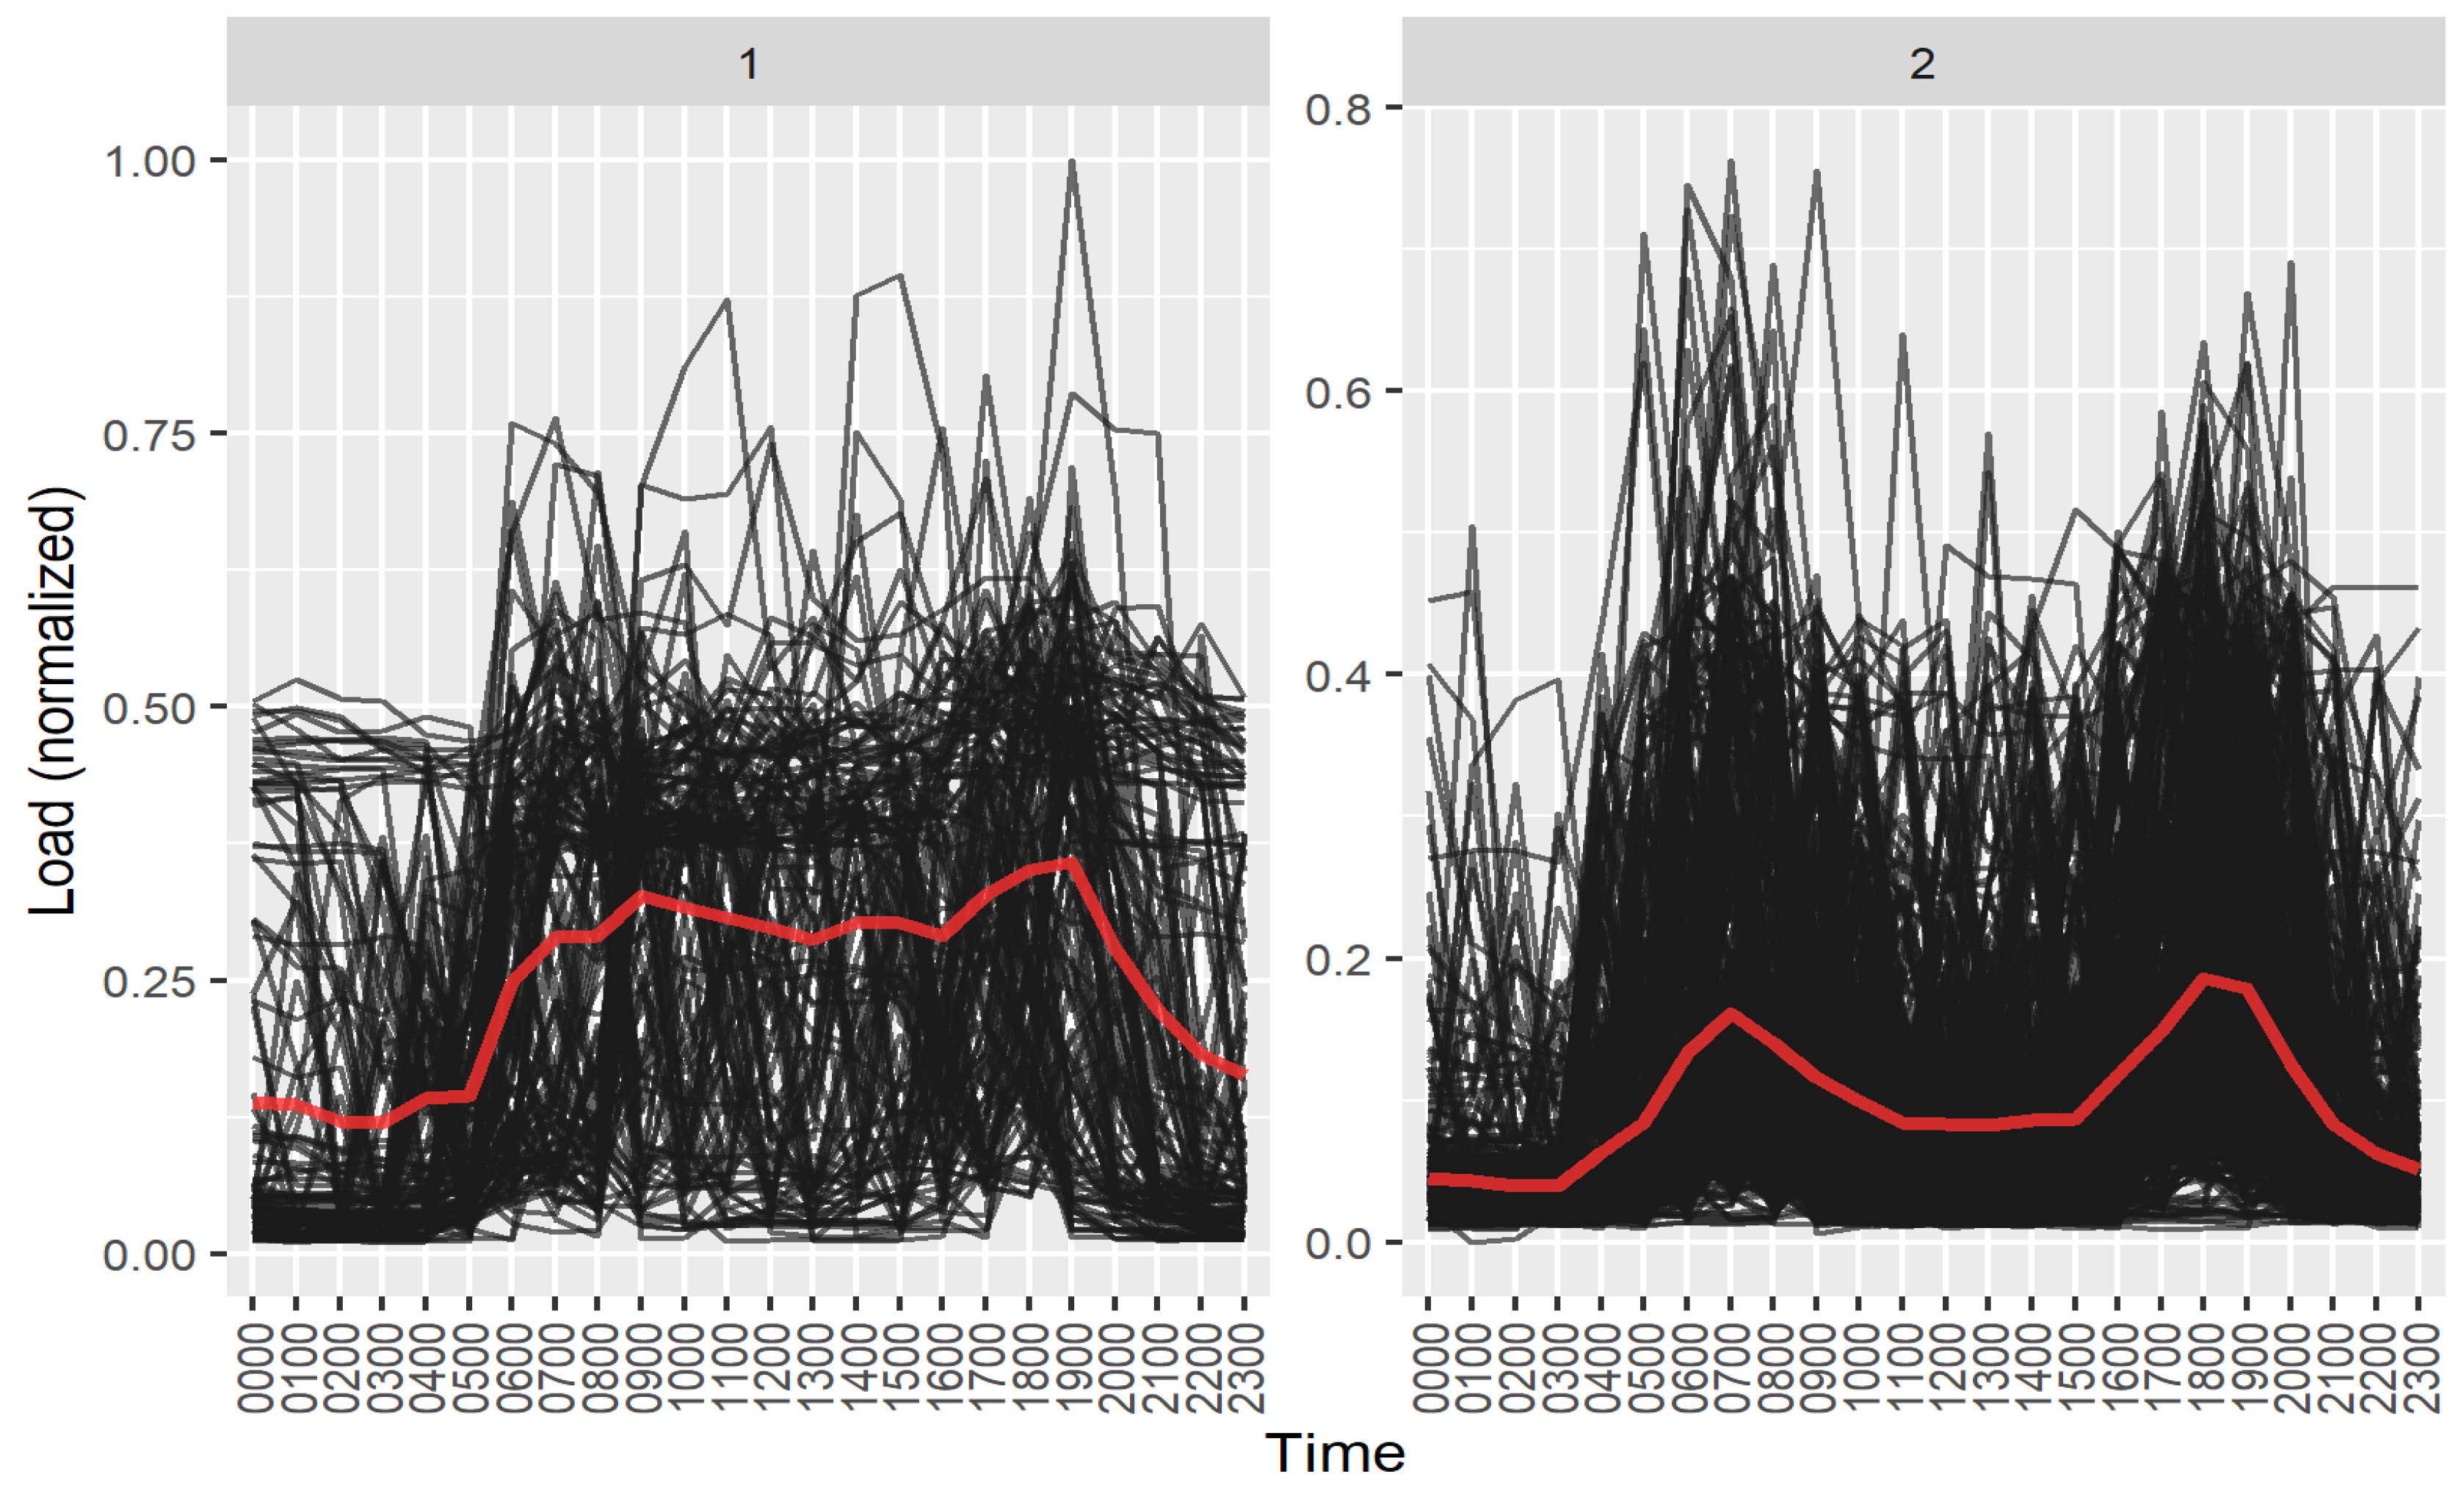
\includegraphics[width=0.8\textwidth]{figures/malatesta_hsop/malatesta_routinisedHousehold.jpg}
    \caption{Single Household Clustering Resulting in a Routinised Household Using all Year Energy Data \cite{MAL-HBP};
    The Red Line represents the Average Consumption in the Cluster, each Black Line represents an assigned Daily Profile;
    X-Axis: Time in 1 Hour Intervals, Y-Axis: Normalized Load Consumption}
    \label{fig:routinized_household}
\end{figure}

\begin{figure}
    \centering
    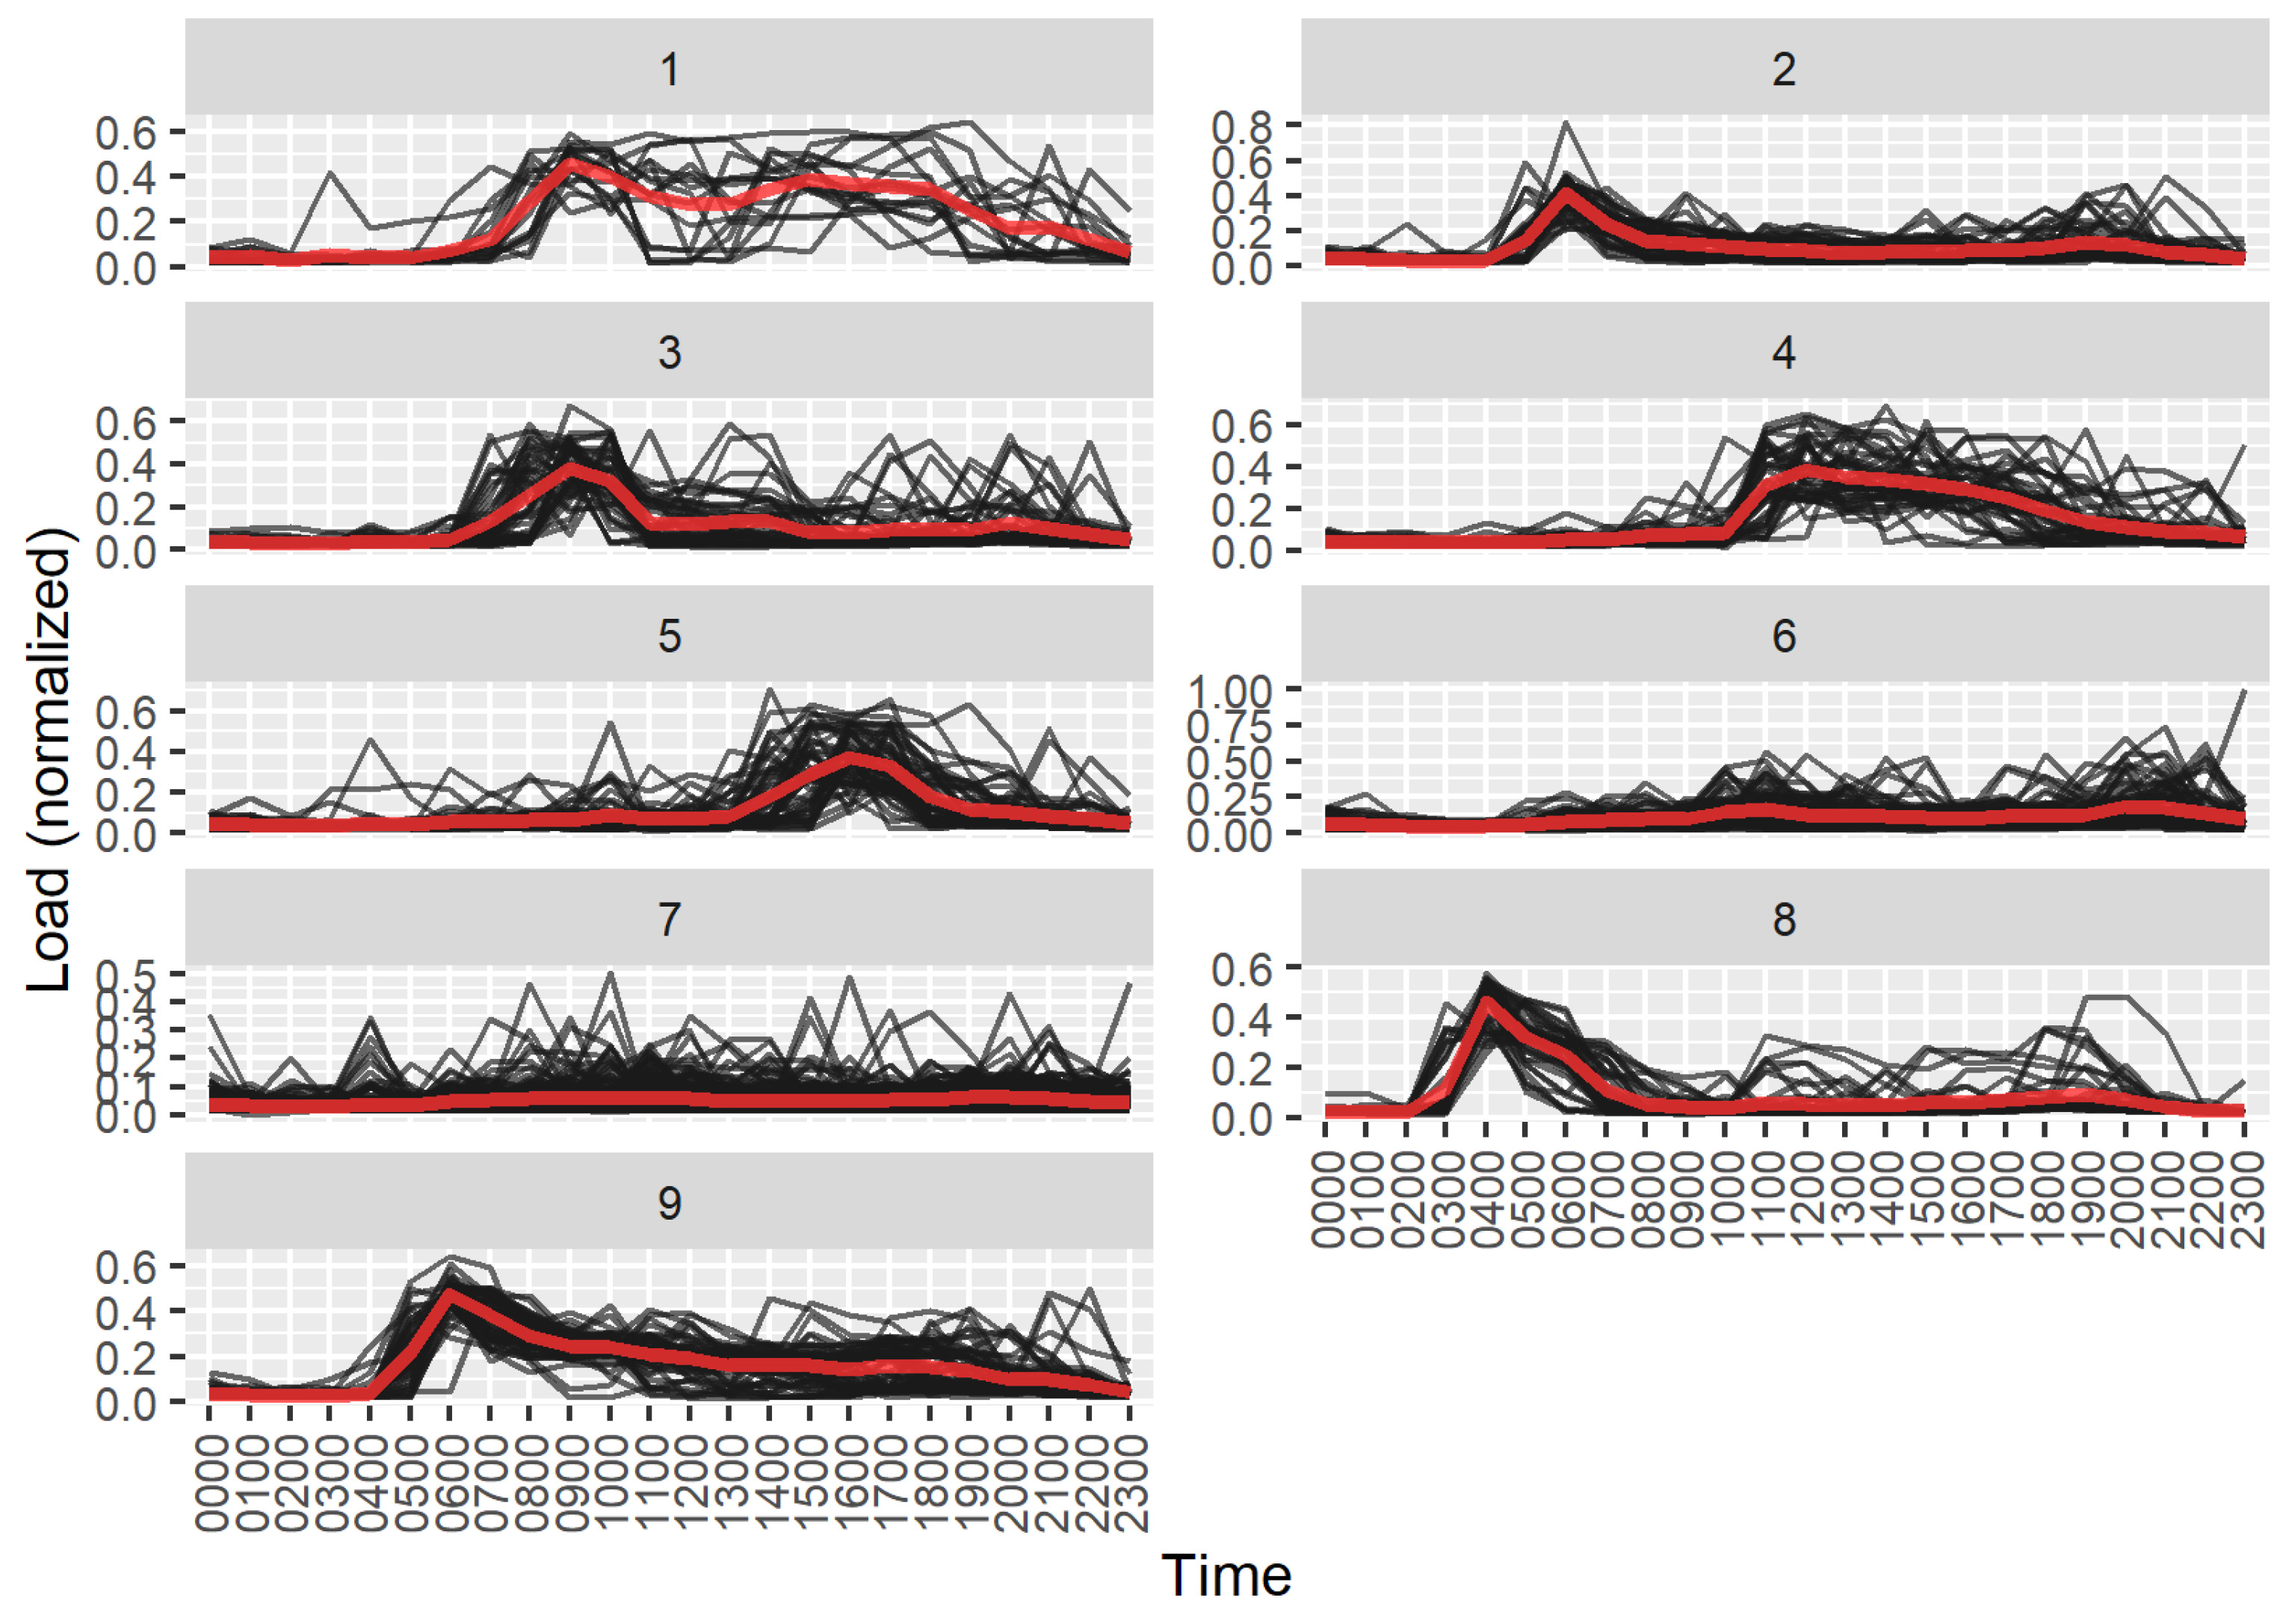
\includegraphics[width=0.8\textwidth]{figures/malatesta_hsop/malatesta_unroutinisedHousehold.jpg}
    \caption{Single Household Clustering Resulting in a Unroutinised Household Using all Year Energy Data \cite{MAL-HBP};
    The Red Line represents the Average Consumption in the Cluster, each Black Line represents an assigned Daily Profile;
    X-Axis: Time in 1 Hour Intervals, Y-Axis: Normalized Load Consumptio}
    \label{fig:non_routinized_household}
\end{figure}

\begin{figure}
    \centering
    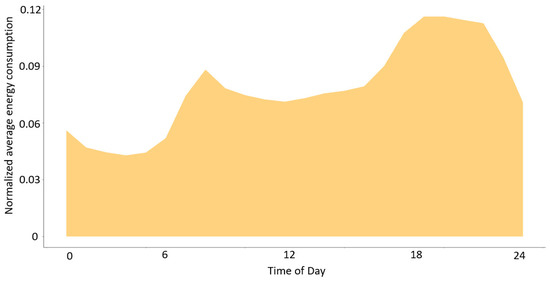
\includegraphics[width=0.8\textwidth]{figures/malatesta_hsop/malatesta_totalDataAveraging.jpg}
    \caption{Result after taking the Average Load Consumption of the Total Dataset \cite{MAL-HBP};
    X-Axis: Time of the Day in Hours, Y-Axis: Normalized Energy Consumption;
    Most Energy Consumption Profiles show a Dual Peak Model with a Dip Midday, the Dominant HSOP}
    \label{fig:total_data_averaging}
\end{figure}

% \paragraph*{MAL-HBP:}
% % Wie soll dieser Paragraph strukturiert sein?
% % 1. Allgemeine Ergebnisse ansprechen
% % 2. Auf ein Beispiel eingehen (in diesem Fall das Clustering und die Tabelle)
% The research is conducted on the total data set and the data split into the disctinct households.
% Also, the data is split into winter and summer data.

% After clustering the whole dataset several assumptions are made.
% First, dominant routines are spotted by averaging the total dataset.
% This leads to a dual peak average as shown in \ref{fig:total_data_averaging}.
% Therefore, practices can be socially shared.
% Also, different consumption practices for the summer and winter seasons are found.

% After applying k-means to each household, routinized households and less routinized households can be identified.
% Routinized households (\ref{fig:routinized_household}) show a smaller number of clusters and therefore less HSOPs than less routinized households (\ref{fig:non_routinized_household}).
% Due to the application of social theories and the survey, two assumptions can be made:
% \begin{itemize}
%     \item Variable lifestyles with different work commitments (e.g. working from home) or family structures (e.g. having children) alter the energy consumption of households \cite{KUR-HBP}.
%     \item If occupants are routinized, their behaviors are repetitive \cite{BRE-EWP}.
% \end{itemize}


% \paragraph*{What do both Summaries have in Common?}
% \begin{itemize}
%     \item Identifying and comparing of:
%     \begin{itemize}
%         % \item Patterns (Malatesta => Habits patterns, clustering of the whole profile; Liu => Some industry sectors are in general more energy consuming than others)
%         % \item Tendencies (Liu => Some industry sectors being represented in cluster 0 and cluster 2)
%         % \item (Best Practices) topic for the conclusion
%         % \item Outliers (Malatesta => Routinised and less routinized households)
%         % \item Shared and individual practices/habits (Malatesta => Whole data clustering)
%         % \item Thresholds (Liu => Limits in consumption/emissions are spotted)
%         \item Characteristics of each cluster (Both => Clusters represent a certain characteristic (Practice/Certain Metric); Malatesta => Some practices can be tracked to a certain practice)
%         \item Dominant characteristics/practices (Malatesta => Some habits reappeared several times in multiple clusterings)
%         % \item Key industries for energy saving incentives (Liu => Some industry sectors are in general more energy consuming than others)
%     \end{itemize}
% \end{itemize}



\paragraph*{Industry:}
% Grundlegende Idee: Ergebnisse in Industrie und Private Housing unterteilen, general findings werden separat für alle Paper gezeigt
% Dabei die jeweiligen Findings am Beispiel zeigen
% Alles was eigentlich aus dem Background klar sein sollte wird dorthin geschoben
% => Nur auf die Ergebnisse aus dem Paper eingehen, dabei nicht werten oder eigene Schlussfolgerungen ziehen
% Die Schritte, wie man zu den Ergebnissen kommt, sollen aus dem Background bereits klar sein
Applying k-means with a fixed value of $k=3$, the datasets are separated into low-, mid-, and highly-efficient industry sectors or companies within these sectors.
Therefore, general patterns are detected and compared.
Spotting these general characteristics' thresholds and characteristic metrics are determined.
A clustering example of the environmental impact measured on $SO_2$ emissions is shown in \ref{fig:multi_industries_clustering_result_environemental_performance}.
General high-consuming, low-efficient industry sectors are spotted, in this case for example the black metal smelting industry as shown in \ref{tab:multi_industries_clustering_results_based_on_the_so2_emission}.
Most clusters are represented in one cluster yet some are scattered over several clusters.
\ref{tab:multi_industries_clustering_results_based_on_the_so2_emission} shows the electric power and heat supply industry as a fitting example.
Mostly this is due to a few companies of the reviewed industry sector being less efficient.
This helps in identifying outliers, which means less efficient sectors and companies.
Therefore, applying k-means to the given dataset helps in finding a starting point in industry sectors and distinct companies for putting energy-saving incentives into action.

\paragraph*{Private Housing:}
Again, patterns are detected using k-means, yet in a different context with different interpretations.
Averaging the whole dataset (\ref{fig:total_data_averaging}) provided insights into dominant practices and habits that are socially shared among the residents of the precinct.
Also, HSOPs are different for the summer and winter seasons due to heating and cooling practices.
These assumptions can be made due to k-means laying the groundwork for applying social theory and the survey results after the clustering process.
The \texttt{dual peak model} with dip midday is the average consumption habit of the monitored precinct.
Analyzing the clustering on the whole dataset gave insights into how habits are shared between different households.
Dominant HSOPs are identified with general characteristics being found.
Clustering single household data gave insights into how flexibility and routine affect different energy consumption practices.
The results varied between two (\ref{fig:routinized_household}) up to nine (\ref{fig:non_routinized_household}) clusters per household.
Due to the application of social theories and surveying the residents, two assumptions are made:
\begin{itemize}
    \item Variable lifestyles with different work commitments (e.g. working from home) or family structures (e.g. having children) alter the energy consumption of households \cite{KUR-HBP}.
    \item If occupants are routinized, their behaviors are repetitive \cite{BRE-EWP}.
\end{itemize}
Therefore, applying k-means to this data reveals the hidden knowledge of HSOPs and identifies starting points for developing best practices in energy consumption.
